\documentclass{VUMIFInfBakalaurinis}
\usepackage{algorithmicx}
\usepackage{algorithm}
\usepackage{algpseudocode}
\usepackage{amsfonts}
\usepackage{amsmath}
\usepackage{bm}
\usepackage{caption}
\usepackage{color}
\usepackage{float}
\usepackage{graphicx}
% \usepackage{hyperref}  % Nuorodų aktyvavimas
\usepackage{listings}
\usepackage{subfig}
\usepackage{url}
\usepackage{wrapfig}

\usepackage{longtable}
\usepackage{rotating}

\definecolor{mygray}{rgb}{0.5,0.5,0.5}
\lstset{ %
  numbers=left,                    % where to put the line-numbers;
  numbersep=5pt,                   % how far the line-numbers are from the code
  numberstyle=\tiny\color{mygray} % the style that is used for the line-numbers 
}


% Titulinio aprašas
\university{Vilniaus universitetas}
\faculty{Matematikos ir informatikos fakultetas}
\department{Programų sistemų katedra}
\papertype{Baigiamasis bakalauro darbas}
\title{Dalykinės srities modelio transformavimas į UML sekų diagramas}
\titleineng{Deriving use cases from business process}
\status{4 kurso 1 grupės studentas}
\author{Aleksandras Sivkovas}
% \secondauthor{Vardonis Pavardonis}   % Pridėti antrą autorių
\supervisor{Prof. dr. Saulius Gudas}
\reviewer{prof. habil. dr. Vardaitis Pavardaitis}
\date{Vilnius \\ \the\year}

% Nustatymai
% \setmainfont{Palemonas}   % Pakeisti teksto šriftą į Palemonas (turi būti įdiegtas sistemoje)
\bibliography{bibliografija} 

\begin{document}
\maketitle

\tableofcontents

%Sutartinių ženklų, simbolių, vienetų ir terminų sutrumpinimų sąrašas (jeigu
%ženklų, simbolių, vienetų ir terminų bendras skaičius didesnis nei 10 ir
%kiekvienas iš jų tekste kartojasi daugiau nei 3 kartus).
\sectionnonum{Sąvokų apibrėžimai}
Šiame darbe naudojami žymėjimai:
\begin{enumerate}
	\item \textbf{BPMN} – modeliavimo kalba, skirta pavaizduoti informaciją plačiai auditorijai. \textbf{BPMN} buvo sukurta ir dažniausia naudojama pavaizduoti verslo procesams \cite{bpmnFormal}.
	\item \textbf{UML} – modeliavimo kalba, skirta suteikti standartinį sistemos analizės, architektūros, veikimo ir kūrimo pavaizdavimą \cite{omgUmlFormal}.
	\item \textbf{Sekų diagrama} – \textbf{UML} diagrama, skirta pavaizduoti žinučių tarp apibrėžtų objektų sekai tų objektų gyvavimo metu \cite{omgUmlFormal}.
	\item \textbf{Vartojimo atvejų diagrama} – \textbf{UML} diagrama, skirta pavaizduoti pavaizduoti kaip gali būti naudojama programų sistema \cite{algUseCasesFromBpmn}.
\end{enumerate}


%Įvade apibūdinamas darbo tikslas, temos aktualumas ir siekiami rezultatai.
\sectionnonum{Įvadas}
Darbo tikslas – apibrėžti ir įgyvendinti algoritmą \textbf{BPMN} modelio transformacijai į \textbf{sekų diagramas}.

Reikalavimų inžinerija yra sudėtinga programų kūrimo dalis. Proceso sudėtingumas dažnai tampa klaidų priežastimi. Čia atsiradusios klaidos sunkiai aptinkamos ir sukelia brangiai kainuojančias pasekmes, nes sekančiuose etapuose bus kuriama neteisingai apibrėžta programa. Norint išvengti klaidų galima kai kurias proceso veiklas automatizuoti.

Darbe bus tiriama verslo proceso transformacija į kuriamos programos \textbf{sekų diagramas}. \textbf{Sekų diagramos} yra svarbi reikalavimų inžinerijos dalis, kadangi ji apibrėžia kokios transakcijos vyks programų sistemoje. Įmonės dažniausiai žino kaip ir kokias veiklas jos vykdo. Verslo procesą galima apibrėžti \textbf{BPMN} diagramomis. Bet ne viską, kas yra \textbf{BPMN} modelyje, galima perkelti į \textbf{sekų diagramą}, todėl darbe bus apibrėžtas modifikuotas \textbf{BPMN} modelis, kuriame bus vaizduojama tik algoritmui aktuali informacija. Taip pat gali tekti pridėti papildomų atributų, kurie padės pasiekti tikslesnius rezultatus. Čia bus tiriama \textbf{BPMN} modelio transformacijos į \textbf{sekų diagramas} algoritmas.

Siekiami rezultatai yra:
\begin{enumerate}
	\item Modifikuoto \textbf{BPMN} modelio apibrėžimas.
	\item Algoritmas galintis transformuoti \textbf{BPMN} modelį į \textbf{sekų diagramą}.
	\item Programa demonstruojanti algoritmo veikimą.
\end{enumerate}


%Pagrindinėje tiriamojoje dalyje aptariama ir pagrindžiama tyrimo metodika;
%pagal atitinkamas darbo dalis, nuosekliai, panaudojant lyginamosios analizės,
%klasifikacijos, sisteminimo metodus bei apibendrinimus, dėstoma sukaupta ir
%išanalizuota medžiaga. 
\section{Tiriamų modelių apibrėžimai}
Kadangi darbe bus tiriama vienos diagramos transformacija į kitą, pirmiausia pateikiami jų apibrėžimai.

%Citavimo pavyzdžiai: cituojamas vienas šaltinis \cite{PvzStraipsnLt}; cituojami
%keli šaltiniai \cite{PvzStraipsnEn, PvzKonfLt, PvzKonfEn, PvzKnygLt, PvzKnygEn,
%PvzElPubLt, PvzElPubEn, PvzMagistrLt, PvzPhdEn}.
\subsection{BPMN diagrama}
\textbf{BPMN} specifikacija leidžia atvaizduoti gana nemažai verslo proceso atributų \cite{bpmnFormal}. Bet šiame darbe ji bus nagrinėjama tik kaip įvesties duomenų formatas, naudojamas apibrėžti informaciją pagal kurią bus kuriama \textbf{sekų diagrama}. Taigi daugelį \textbf{BPMN} komponentų galima tiesiog ignoruoti, nes jie neturi jokios įtakos algoritmo vykdymo rezultatui. Norint pabrėžti svarbią informaciją, darbe bus tiriamos tik tos \textbf{BPMN} savybės kurios gali įtakoti algoritmo vykdymo rezultatą. Atitinkami komponentai pavaizduoti \ref{tab:investigated_bpmn_components} lentelėje.
\newcounter{counter:table:reset}
\newcounter{counter:table}[counter:table:reset]
\newcommand\rownumber{\stepcounter{counter:table}\arabic{counter:table}}
\begin{center}
    \begin{longtable}{ | p{0.5cm} | p{2cm} |  p{7cm} | p{4cm} |}
    \caption{BPMN diagramos komponentai}
	\label{tab:investigated_bpmn_components}
    \\ \hline 
    Nr. & Komponentas & Aprašymas & Žymėjimo pavizdys\\ 
    \hline 
    \rownumber & Rolė & Komponentas žymintis diagramos dalyvį ir nurodantis, kad jis atsakingas už veiklų esančių šiame komponente vykdymą. & \vtop{\hbox{\strut }\hbox{\strut 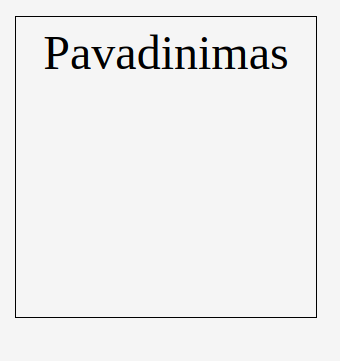
\includegraphics[width=3cm]{img/bpm-components/pool}}} \\
    \hline
     \rownumber & Įvykis & Komponentas žymintis, kad ivyko kažkas kas įtakojo proceso būseną. & \vtop{\hbox{\strut }\hbox{\strut 
\includegraphics[width=3cm]{img/bpm-components/event}}} \\ 
    \hline 
    \rownumber & Veikla & Komponentas žymintis užduoties vykdymo procesą & \vtop{\hbox{\strut }\hbox{\strut 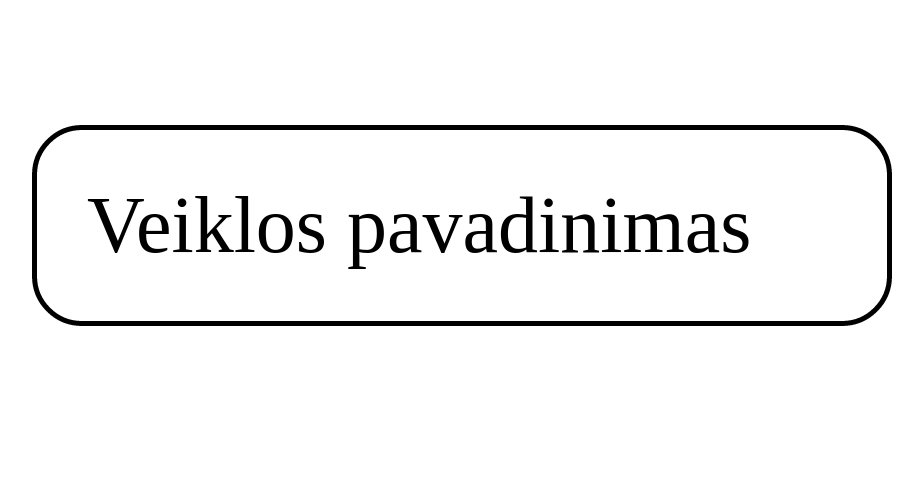
\includegraphics[width=3cm]{img/bpm-components/activity}}}\\
    \hline 
    \rownumber & Sekos srautas & Komponentas žymintis veiklų seką. & \vtop{\hbox{\strut }\hbox{\strut 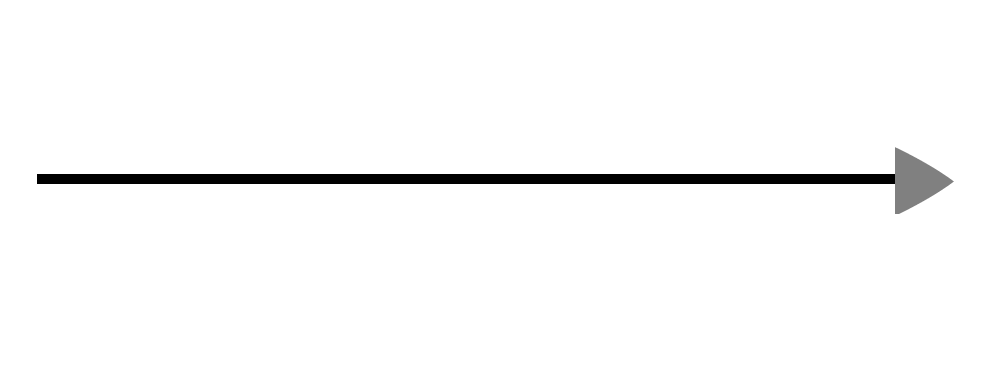
\includegraphics[width=3cm]{img/bpm-components/transition}}}\\
    \hline
    \rownumber & Duomenų objektas & Komponentas žymintis sukuriamus arba įeities duomenis. & \vtop{\hbox{\strut }\hbox{\strut 
\includegraphics[width=3cm]{img/bpm-components/data_object}}}\\
    \hline
    \rownumber & Pranešimų srautas & Komponentas žymintis duomenų apsikeitimo srautus. & \vtop{\hbox{\strut }\hbox{\strut 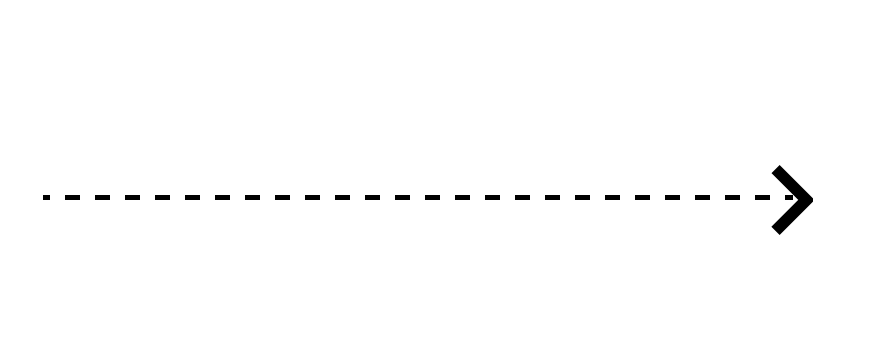
\includegraphics[width=3cm]{img/bpm-components/message_flow}}}\\
    \hline
    \rownumber & Sprendimas & Komponentas žymintis sekos srautų išsišakojimą. & \vtop{\hbox{\strut }\hbox{\strut 
\includegraphics[width=3cm]{img/bpm-components/gateway}}}\\
    \hline
    \end{longtable}
\end{center}


\subsection{Sekų diagrama}

Kaip ir \textbf{BPMN} atveju \textbf{sekų diagrama} turi komponentus, kurie nebus nagrinėjami šiame darbe. \ref{tab:investigated_sequence_diagram_components} lentelė vaizduoja kas bus tiriama iš \textbf{sekų diagramos}.
\stepcounter{counter:table:reset}
\begin{center}
    \begin{longtable}{ | p{0.5cm} | p{2cm} |  p{7cm} | c |}
    \caption{Sekų diagramos komponentai}
	\label{tab:investigated_sequence_diagram_components}
    \\ \hline 
    Nr. & Komponentas & Aprašymas & Žymėjimo pavizdys\\ 
    \hline 
    \rownumber & Gyvavimo linija & Komponentas žymintis diagramos objekto dalyvavimo laiką procese. & \vtop{\hbox{\strut }\hbox{\strut 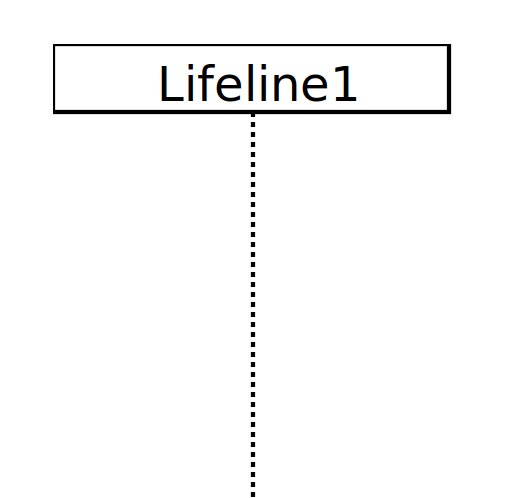
\includegraphics[width=3cm]{img/sequence-diagram-components/lifeline}}} \\
    \hline
    \rownumber & Vykdymo specifikacija & Komponentas žymintis sinchroninio pranešimo tranzakciją. & \vtop{\hbox{\strut }\hbox{\strut 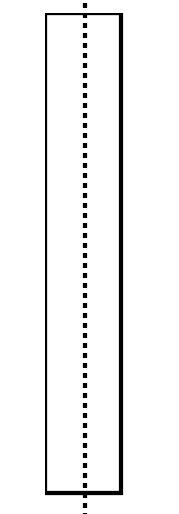
\includegraphics[height=3cm]{img/sequence-diagram-components/execution_specification}}} \\
    \hline
     \rownumber & Žinutė & Komponentas žymintis duomenų perdavimą iš vieno dalyvio į kitą & \vtop{\hbox{\strut }\hbox{\strut 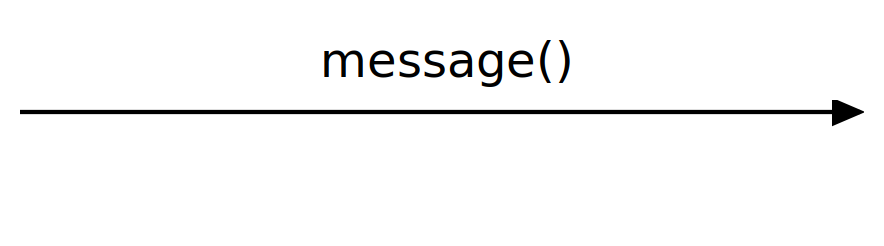
\includegraphics[width=3cm]{img/sequence-diagram-components/message}}} \\
    \hline
     \rownumber & Atsakymas & Komponentas žymintis, kad dalyvis sureagavo į sinchroninę užduotį. & \vtop{\hbox{\strut }\hbox{\strut 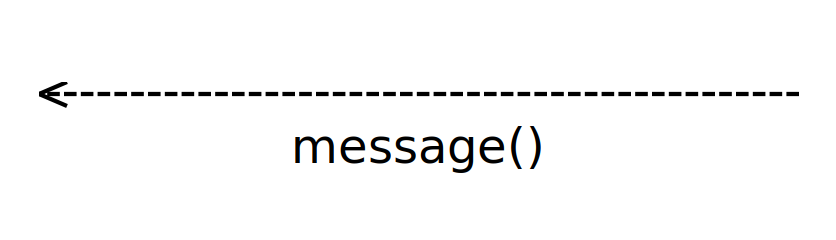
\includegraphics[width=3cm]{img/sequence-diagram-components/reply-message}}} \\
    \hline
    \end{longtable}
\end{center}

\section{Algoritmas kurti \textbf{sekų diagramas} pagal \textbf{BPMN} pateiktą informaciją}
Šio darbo tikslas yra algoritmas atlikti diagramų transformacijai. Pirmiausia pateikiama tai, kas literatūroje rašoma apie \textbf{UML} diagramų transformavimo algoritmus. Vėliau sukuriamas siekiamas algoritmas.
\subsection{\textbf{UML} diagramų transformavimo algoritmai}
\subsubsection{\textbf{Vartojimo atvejų diagramos} išvedimas iš \textbf{BPMN} modelio} \label{section:use_cases_from_bpmn}
Literatųroje yra parašyta apie \textbf{vartojimo atvejų diagramos} išvedimą iš \textbf{BPMN} modelio \cite{algUseCasesFromBpmn}. Darbe nagrinėjamas \cite{algUseCasesFromBpmn} straipsnyje aprašytas algoritmas (\ref{eq:use_cases_from_bpmn}). Imamas modifikuotas \textbf{BPMN} modelis (\ref{eq:use_cases_from_bpmn:bpmn_elements}) ir tie \textbf{vartojimo atvejų diagramos} komponentai, kurie gali būti iš jo išvesti (\ref{eq:use_cases_from_bpmn:use_case_elements}). 
\begin{align}
&BPMNElements = \left\{Start,End,Role,Branch,Task,Transition\right\}; \label{eq:use_cases_from_bpmn:bpmn_elements} \\
\begin{split}
&UseCasesElements = \left\{Actor, Generalization, Association,Use Case,\right. \\
&\left. Include, Extension Point, Extend\right\}; \label{eq:use_cases_from_bpmn:use_case_elements}\\
\end{split} \\
&BPMN(BPMNModelElements) \Rightarrow UseCases(UseCasesElements); \label{eq:use_cases_from_bpmn}
\end{align}

Algoritmo autoriai pirmiausia siūlo surasti ryšius tarp modelių. Rolės atitinka aktorius. Užduotys tuo tarpu grupuojamos, kol nepasiekia maksimalaus skaičiaus vykdomų be pertraukos, tos pačios rolės ir pagaminančių rezultatą. Tokia grupė pavadinama žingsniu ir yra laikoma atitinkančia vartojimo atvejį. Taip  išsiaiškinami transformacijos žingsniai. Tuomet lieka tik formaliai užrašyti kaip jie gali būti vykdomi ir surasti kaip dar galima būtų panaudoti informaciją, patikslinti ir suprastinti gautoms diagramoms.

Algoritmas Pirmiausia sudėlioja pavienes užduotis į proceso žingsnius. Vėliau Rolės tampa aktoriais, o žingsniai jose – vartojimo atvejais. Galiausiai pasikartojančios užduotis išimamos iš žingsnių ir prijungiamos asociacija įtraukia arba išplečia pagal situaciją.


\subsection{Sekų diagramos išvedimas iš \textbf{BPMN} modelio}

Šio darbo tikslas, algoritmas galintis gauti \textbf{sekų diagramas} iš \textbf{BPMN} modelio, bus kuriamas pagal \ref{section:use_cases_from_bpmn} aprašytą algoritmo sukūrimo pavyzdį. Pirmiausia bus rasti ryšiai tarp diagramų, vėliau sukurtas būdas juos panaudoti, galiausiai panaudota likusi modelio informacija patikslinti ir suprastinti diagramoms.

\subsubsection{Ryšiai tarp \textbf{BPMN} ir \textbf{sekų diagramų}} \label{section:relations_sd_bpmn}

Norint duomenis iš vieno modelio perkelti į kitą galima pasinaudoti ryšiais esančiais tarp jų.

\begin{center}
    \begin{longtable}{ | c | c |  c | c | c |}
    \caption{Ryšiai tarp \textbf{BPMN} ir \textbf{sekų diagramų}}
	\label{tab:relations_sd_bpmn}
    \\ \hline 
     & 
     %\begin{turn}{-90}
     Gyvavimo linija 
     %\end{turn} 
     & 
     %\begin{turn}{-90}
     Vykdymo specifikacija 
     %\end{turn}  
     & 
     %\begin{turn}{-90}
     Žinutė 
     %\end{turn}  
     & 
     %\begin{turn}{-90}
     Atsakymas 
     %\end{turn} 
     \\ 
    \hline 
    Rolė & + & + & + & + \\
    \hline
    Įvykis  & & + & + & \\
    \hline 
    Veikla  & & + & + & + \\
    \hline 
    Sekos srautas  & & + & + & \\
    \hline
    Duomenų objektas  & & & + & +\\
    \hline
    Pranešimų srautas  & & & + & +\\
    \hline
    Sprendimas  & & & & \\
    \hline
    \end{longtable}
\end{center} 

TODO: Vykdymo specifikacija.(turbūt išvestinis komponentas ir jo skaičiuoti nereikia)

Sprendimas neturi ryšiu su \textbf{sekų diagramos} komponentais, bet jis nėra nesusijęs su ja. Kiekvienas išeinantis sekos srautas sprendime reiškia naują \textbf{sekų diagramą}. 
\begin{enumerate}
	\item Gyvavimo linija – galima gauti iš informacijos esančios rolėje. 
	\item Žinutė – Daugiausia informacijos reikalaujantis komponentas. Ją galima apibrėžti kaip sekos srauto perėjimą iš vienos rolės kitai, kai įvyksta įvykis arba kuri nors rolė atliko savo veiklų seką ir tęsti darbui reikalingos kitos rolės įvykdytos veiklos. Šis veiksmas dažniausiai taip pat reikalauja Duomenų objekto keliaujančio duomenų srautu.
	\item Atsakymas – duomenų objektas keliaujantis pranešimų srautu iš vienos veiklos esančios rolėje į kitą.
	\item Vykdymo specifikacija – Atsiranda, kai rolėje vyksta sekos srauto perėjimas tarp jo jungiamų komponentų.
\end{enumerate} 

\subsubsection{Ryšių tarp diagramų panaudojimas transformacijai}

Rasti ryšiai parodo į kokius \textbf{BPMN} komponentus reikia žiūrėti kuriant \textbf{sekų diagramos} dalis. Toliau sudėliojami konkretūs žingsniai kuriuos reikia atlikti. Galiausiai gaunamas pseudokodas \ref{lst:bpmn_to_sd_algorythm_pseudocode}. 

\begin{enumerate}
	\item Pirmiausia sukuriama proceso gyvavimo linija ir jos vykdymo specifikacija. Ji tęsis visą vykdymą, perduos informaciją, gautą iš vienų dalyvių kitiem. 
	\item Vėliau iš rolių informacijos gaunamos gyvavimo linijos. Galiausiai randama pirmoji proceso veikla \lstinline[columns=fixed]{sequenceFlows.filter(flow => flow.from.type == start)[0];}. Ir pradedant nuo jos, visos veiklos paverčiamos į žinutes, kurios siunčiamos iš proceso vykdymo specifikacijos į naują vykdymo specifikaciją sukurtą gyvavimo linijoje, kuri buvo sukurta iš informacijos rolėje kuriai priklauso duota veikla. Žinutės įvesties parametrais tampa duomenų objektai, kurių duomenų srautas rodo į nagrinėjamą veiklą. Išvestis gaunama iš duomenų objektų, kurių duomenų srautas veda iš nagrinėjamos veiklos. 
	\item Atsakymas gaunamas iš duomenų žinutėje, nes jis yra susijęs su ja. 
\end{enumerate} 

\begin{lstlisting}[language=java, caption={\textbf{UML} \textbf{Sekų diagramos} gavimo iš \textbf{BPMN} modelio algoritmo pseudokodas}, label={lst:bpmn_to_sd_algorythm_pseudocode}]
{roles,events,activities, sequenceFlows,messageFlows,decisions} = BPMN;

lifelines = [];
processLifeline = new Lifeline(BPMN.name);
processExecutionSpecification = processLifeline.createExecutionSpecification();
lifelines.push(processLifeline);
rolesLifelinesMap = new Map();
for(role in roles){
	lifeline = createLifeline(role);
	rolesLifelinesMap.set(role,lifeline);
	lifelines.add(lifeline);
}
syncMessages = [];
returnMessages = [];
startFlow = sequenceFlows.filter(flow => flow.from.type == start)[0];
for(
	flow = startFlow;
	flow.from.type != end;
	flow = sequenceFlows.filter(flow => flow.from.equals(activity))[0]
){
	activity = flow.to;
	lifeline = rolesLifelinesMap.get(activity.role);
	executionSpecification = lifeline.createExecutionSpecification();
	
	inputDataFlows = messageFlows.filter(flow => flow.to.equals(activity));
	inputParameters = inputDataFlows.map(flow => flow.from);
	
	outputDataFlow = messageFlows.filter(flow => flow.from.equals(activity))[0];
	returnParameter = 	outputDataFlow.to;
	
	
	message = createSyncMessage(
			processExecutionSpecification,
			executionSpecification,
			activity.name,
			inputParameters,
			returnParameter
	);
	syncMessages.push(message);	
	
	returnMessage = createReturnMessage(message);
	returnMessages.push(returnMessage);	
}
sequenceDiagram = {lifelines,syncMessages,returnMessages};
\end{lstlisting}

\subsubsection{Likusios informacijos panaudojimas suprastinti ar patikslinti diagramai}


\section{Programa \textbf{BPMN} transformacijai į \textbf{sekų diagramą}}   


%Išvadose ir pasiūlymuose, nekartojant atskirų dalių apibendrinimų,
%suformuluojamos svarbiausios darbo išvados, rekomendacijos bei pasiūlymai.
\sectionnonum{Išvados}

%Šiame skyriuje pateikiamos išvados (reziume) anglų kalba.
\sectionnonum{Conclusions}


% bibliografija.bib faile. Šaltinių sąraše nurodoma panaudota literatūra,
% kitokie šaltiniai. Abėcėlės tvarka išdėstoma tik darbe panaudotų (cituotų,
% perfrazuotų ar bent paminėtų) mokslo leidinių, kitokių publikacijų
% bibliografiniai aprašai (šiuo punktu pasirūpina LaTeX). Aprašai pateikiami
% netransliteruoti.
\printbibliography[heading=bibintoc] % Literatūros šaltiniai aprašomi


% Prieduose gali būti pateikiama pagalbinė, ypač darbo autoriaus savarankiškai
% parengta, medžiaga. Savarankiški priedai gali būti pateikiami kompiuterio
% diskelyje ar kompaktiniame diske. Priedai taip pat vadinami ir numeruojami.
% Tekstas su priedais siejamas nuorodomis (pvz.: \ref{img:mlp}).
\appendix  % Priedai


%\section{Niauroninio tinklo struktūra}
%\begin{figure}[H]
%    \centering
%    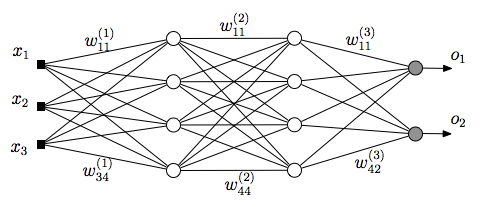
\includegraphics[scale=0.5]{img/MLP}
%    \caption{Paveikslėlio pavyzdys}
%    \label{img:mlp}
%\end{figure}


%\section{Eksperimentinio palyginimo rezultatai}
% tablesgenerator.com - converts calculators (e.g. excel) tables to LaTeX
%\begin{table}[H]\footnotesize
%  \centering
%  \caption{Lentelės pavyzdys}
%  {\begin{tabular}{|l|c|c|} \hline
%    Algoritmas & $\bar{x}$ & $\sigma^{2}$ \\
%    \hline
%    Algoritmas A  & 1.6335    & 0.5584       \\
%    Algoritmas B  & 1.7395    & 0.5647       \\
%    \hline
%  \end{tabular}}
%  \label{tab:table example}
%\end{table}

\end{document}
